\let\lesson\undefined
\newcommand{\lesson}{\phantomlesson{Bài 18.}}
\setcounter{section}{2}
\section{Trắc nghiệm nhiều phương án lựa chọn}
\setcounter{ex}{0}
\Opensolutionfile{ans}[ans/VN10-Y24-PH-SYL-029P-TN]
% ===================================================================
\begin{ex}\mkstar{2}
	Động lượng là đại lượng vector
	\choice
	{\True cùng phương, cùng chiều với vectơ vận tốc}
	{cùng phương, ngược chiều với vectơ vận tốc}
	{có phương vuông góc với vectơ vận tốc}
	{có phương hợp với vectơ vận tốc một góc $\alpha$ bất kì}
	\loigiai{Động lượng là đại lượng vector cùng phương, cùng chiều với vectơ vận tốc.}
\end{ex}
% ===================================================================
\begin{ex}\mkstar{2}
		Chọn câu phát biểu \textbf{sai}?
	\choice
	{Động lượng là một đại lượng vector}
	{Động lượng luôn được tính bằng tích khối lượng và vận tốc của vật}
	{\True Động lượng luôn cùng hướng với vận tốc vì vận tốc luôn luôn dương}
	{Động lượng luôn cùng hướng với vận tốc vì khối lượng luôn luôn dương}
	\loigiai{}
\end{ex}
% ===================================================================
\begin{ex}\mkstar{2}
	Hai vật có khối lượng $m_1 = 2m_2$, chuyển động với vận tốc có độ lớn $v_1 = 2v_2$. Độ lớn động lượng của hai vật có quan hệ
	\choice
	{$p_1=2p_2$}
	{\True $p_1=4p_2$}
	{$p_2=4p_1$}
	{$p_1=p_2$}
	\loigiai{$$\dfrac{p_1}{p_2}=\dfrac{m_1v_1}{m_2v_2}=4.$$}
\end{ex}

% ===================================================================
\begin{ex}\mkstar{2}
	Một vật có khối lượng $\SI{500}{\gram}$ chuyển động theo chiều âm của trục toạ độ $Ox$ với tốc độ $\SI{12}{\meter/\second}$. Động lượng của vật có giá trị là
	\choice
	{$\SI{6}{\kilogram\cdot\meter/\second}$}
	{$\SI{-3}{\kilogram\cdot\meter/\second}$}
	{\True $\SI{-6}{\kilogram\cdot\meter/\second}$}
	{$\SI{3}{\kilogram\cdot\meter/\second}$}
	\loigiai{Động lượng của vật:
		$$p=mv=\left(\SI{0.5}{\kilogram}\right)\cdot\left(\SI{-12}{\meter/\second}\right)=\SI{-6}{\kilogram\cdot\meter/\second}.$$}
\end{ex}
% ===================================================================
\begin{ex}\mkstar{2}
Một electron chuyển động với tốc độ $\xsi{2\cdot 10^7}{m/s}$. Biết khối lượng electron bằng $\text{9,1} \cdot 10^{-31}\ \text{kg}.$ Động lượng của electron bằng	
	\choice
	{\True $\SI{1.82E-23}{\kilogram\cdot\meter/\second}$}
	{$\SI{8.2E-23}{\kilogram\cdot\meter/\second}$}
	{$\SI{1.2E-23}{\kilogram\cdot\meter/\second}$}
	{$\SI{1.6E-23}{\kilogram\cdot\meter/\second}$}
	\loigiai{Động lượng của electron
		$$ p  = mv = \text{1,82}\xsi{\cdot 10^{-23}}{\kilogram\cdot\meter/\second}.$$}
\end{ex}
% ===================================================================
\begin{ex}\mkstar{2}
Một quả bóng nặng $\SI{1}{kg}$ đang đứng yên thì cầu thủ chạy đến sút quả bóng thật mạnh. Quả bóng bay đi với vận tốc $\SI{25}{m/s}$. Động lượng của quả bóng có giá trị là
			\choice
			{$\SI{15}{kg.m/s}$}
			{$\SI{2}{kg.m/s}$}
			{$\SI{5}{kg.m/s}$}
			{\True $\SI{25}{kg.m/s}$}
			\loigiai{Động lượng của quả bóng: $p=mv=\SI{25}{kg.m/s}$.}
		\end{ex}
% ===================================================================
\begin{ex}\mkstar{3}
Một chất điểm chuyển động không vận tốc đầu dưới tác dụng của lực không đổi $F =\SI{1}{\newton}$. Động lượng của chất điểm ở thời điểm $t = \SI{3}{\second}$ kể từ lúc bắt đầu chuyển động là	
	\choice
	{$\SI{30}{\kilogram\cdot\meter/\second}$}
	{\True $\SI{3}{\kilogram\cdot\meter/\second}$}
	{$\SI{0.3}{\kilogram\cdot\meter/\second}$}
	{$\SI{0.03}{\kilogram\cdot\meter/\second}$}
	\loigiai{Động lượng của chất điểm ở thời điểm $t=\SI{3}{\second}$:
		$$p=F\cdot t=\SI{3}{\kilogram\cdot\meter/\second}.$$}
\end{ex}
% ===================================================================
\begin{ex}\mkstar{3}
	Một quả bóng có khối lượng $m$ đang bay ngang với vận tốc $v$ thì đập vào một bức tường rồi bật trở lại với cùng tốc độ. Nếu chọn chiều dương cùng chiều chuyển động lúc đầu của quả bóng thì xung lượng của lực gây ra bởi tường lên quả bóng là
	\choice
	{$mv$}
	{$-mv$}
	{$2mv$}
	{\True $-2mv$}
	\loigiai{Xung lượng của lực gây ra bởi tường lên quả bóng:
		$$F\Delta t=\Delta p=m\cdot\left(-v\right)-mv=-2mv.$$}
\end{ex}
% ===================================================================
\begin{ex}\mkstar{3}
Một quả bóng golf có khối lượng $\SI{46}{\gram}$ đang nằm yên, sau một cú đánh quả bóng bay lên với tốc độ $\SI{70}{\meter/\second}$. Tính độ lớn trung bình của lực tác dụng vào quả bóng. Biết thời gian tác dụng là $\SI{0.5E-3}{\second}$.	
	\choice
	{\True $\SI{6400}{\newton}$}
	{$\SI{600}{\newton}$}
	{$\SI{400}{\newton}$}
	{$\SI{3400}{\newton}$}
	\loigiai{Xung lượng của lực
		$$\Delta \vec p = \vec {p'} - \vec p \Rightarrow \Delta p = \SI{3,22}{kgm/s}.$$
		Lực tác dụng vào quả bóng
		$$F = \dfrac{\Delta p}{\Delta t} = \SI{6400}{N}.$$}
\end{ex}
% ===================================================================
\begin{ex}\mkstar{3}
	Viên đạn có khối lượng $\SI{20}{\gram}$ đang bay với tốc độ $\SI{600}{\meter/\second}$ thì gặp một cánh cửa thép. Đạn xuyên qua cửa trong thời gian $\SI{0.002}{\second}$. Sau khi xuyên qua cánh cửa tốc độ của đạn còn $\SI{300}{\meter/\second}$. Lực cản trung bình của cửa tác dụng lên đạn có độ lớn bằng
	\choice
	{\True $\SI{3000}{\newton}$}
	{$\SI{900}{\newton}$}
	{$\SI{9000}{\newton}$}
	{$\SI{30000}{\newton}$}
	\loigiai{Lực cản trung bình của cửa tác dụng lên đạn:
		$$F_c=\dfrac{\Delta p}{\Delta t}=\dfrac{m\Delta v}{\Delta t}=\dfrac{\left(\SI{0.02}{\kilogram}\right)\cdot\left(\SI{-300}{\meter/\second}\right)}{\SI{0.002}{\second}}=\SI{-3000}{\newton}.$$}
\end{ex}
% ===================================================================
\begin{ex}\mkstar{3}
	Cho hệ hai vật có khối lượng bằng nhau $m_1 = m_2 = \SI{1}{\kilogram}$. Vận tốc của vật 1 có độ lớn $v_1 =\SI{1}{\meter/\second}$, vận tốc của vật 2 có độ lớn $v_2 =\SI{2}{\meter/\second}$. Khi vectơ vận tốc của hai vật cùng hướng với nhau, tổng động lượng của hệ có độ lớn là
	\choice
	{$\SI{1}{\kilogram\cdot\meter/\second}$}
	{$\SI{2}{\kilogram\cdot\meter/\second}$}
	{\True $\SI{3}{\kilogram\cdot\meter/\second}$}
	{$\SI{0.5}{\kilogram\cdot\meter/\second}$}
	\loigiai{Động lượng của hệ:
		$$\vec p=\vec p_1+\vec p_2$$
		Vì $\vec p_1\uparrow\uparrow\vec p_2$ nên:
		$$p=p_1+p_2=m_1v_1+m_2v_2=\SI{3}{\kilogram\cdot\meter/\second}.$$}
\end{ex}
% ===================================================================
\begin{ex}\mkstar{3}
	Hai vật có khối lượng $m_1=\SI{2}{\kilogram}$ và $m_2=\SI{3}{\kilogram}$ chuyển động ngược chiều nhau với tốc độ lần lượt bằng $\SI{8}{\meter/\second}$ và $\SI{4}{\meter/\second}$. Độ lớn tổng động lượng của hệ bằng
	\choice
	{$\SI{16}{\kilogram\cdot\meter/\second}$}
	{$\SI{12}{\kilogram\cdot\meter/\second}$}
	{$\SI{30}{\kilogram\cdot\meter/\second}$}
	{\True $\SI{4}{\kilogram\cdot\meter/\second}$}
	\loigiai{Động lượng của hệ:
		$$\vec p=\vec p_1+\vec p_2$$
		Vì $\vec p_1 \uparrow\downarrow \vec p_2$ nên:
		$$p=\left|m_2v_2-m_1v_1\right|=\SI{4}{\kilogram\cdot\meter/\second}.$$}
\end{ex}
% ===================================================================
\begin{ex}\mkstar{3}
	Một hệ gồm 2 vật có khối lượng $m_1 = \SI{1}{\kilogram}$, $m_2 =\SI{4}{\kilogram}$, có vận tốc lần lượt là $v_1 = \SI{3}{\meter/\second}$, $v_2=\SI{1}{\meter/\second}$. Biết 2 vật chuyển động theo hướng vuông góc nhau. Độ lớn động lượng của hệ là
	\choice
	{\True $\SI{5}{\kilogram\cdot\meter/\second}$}
	{$\SI{10}{\kilogram\cdot\meter/\second}$}
	{$\SI{20}{\kilogram\cdot\meter/\second}$}
	{$\SI{14}{\kilogram\cdot\meter/\second}$}
	\loigiai{Động lượng của hệ:
		$$\vec p=\vec p_1+\vec p_2$$
		Vì $\vec p_1 \bot \vec p_2$ nên:
		$$p=\sqrt{p^2_1+p^2_2}=\SI{5}{\kilogram\cdot\meter/\second}.$$}
\end{ex}
% ===================================================================
\begin{ex}\mkstar{3}
Cho hệ hai vật có khối lượng bằng nhau $m_1 = m_2 =\SI{1}{\kilogram}$. Vận tốc của vật 1 có độ lớn $v_1 =\SI{1}{\meter/\second}$, vận tốc của vật 2 có độ lớn $v_2 =\SI{2}{\meter/\second}$. Khi vectơ vận tốc của hai vật hợp với nhau một góc $\SI{60}{\degree}$ thì tổng động lượng của hệ có độ lớn là	
	\choice
	{\True $\SI{2.65}{\kilogram\cdot\meter/\second}$}
	{$\SI{26.5}{\kilogram\cdot\meter/\second}$}
	{$\SI{28.9}{\kilogram\cdot\meter/\second}$}
	{$\SI{2.89}{\kilogram\cdot\meter/\second}$}
	\loigiai{Động lượng của hệ:
		$$\vec p=\vec p_1+\vec p_2$$
		Vì $\left(\vec p_1, \vec p_2\right)=\SI{60}{\degree}$ nên:
		$$p=\sqrt{p^2_1+p^2_2+2p_1p_2\cos\SI{60}{\degree}}\approx\SI{2.65}{\kilogram\cdot\meter/\second}.$$}
\end{ex}
\Closesolutionfile{ans}
\section{Trắc nghiệm đúng/sai}
\setcounter{ex}{0}
\Opensolutionfile{ans}[ans/VN10-Y24-PH-SYL-029P-TF]
% ===================================================================
\begin{ex}\mkstar{2}
	Một vật có khối lượng $m=\SI{800}{\gram}$, chuyển động trên trục $Ox$ và có phương trình vận tốc $v=-5+2t$ ($v$ tính bằng $\si{\meter/\second}$, $t$ tính bằng giây).
	\choiceTF[t]
	{Động lượng của vật có độ lớn luôn tăng theo thời gian}
	{Động lượng của vật tại thời điểm $t=0$ có giá trị bằng $\SI{4}{\kilogram\cdot\meter/\second}$}
	{\True Động lượng của vật tại thời điểm $t=\SI{2.5}{\second}$ bằng 0}
	{\True Độ biến thiên động lượng của vật kể từ thời điểm $t_0=0$ đến thời điểm $t_1=\SI{4}{\second}$ bằng $\SI{6.4}{\kilogram\cdot\meter/\second}$}
	\loigiai{}
\end{ex}
% ===================================================================
\begin{ex}\mkstar{3}
Một quả bóng có khối lượng $m=\SI{300}{\gram}$ va chạm vào tường và nảy trở lại với cùng tốc độ. Tốc độ quả bóng trước va chạm là $\SI{5}{\meter/\second}$. Chọn chiều dương là chiều của quả bóng bay vào tường.
	\choiceTF[t]
	{\True Động lượng của vật trước khi chạm vào tường là $\SI{1.5}{\kilogram\cdot\meter/\second}$}
	{\True Vận tốc quả bóng lúc bật lại có giá trị $\SI{-5}{\meter/\second}$}
	{\True Động lượng của vật khi bật lại có giá trị là $\SI{-1.5}{\kilogram\cdot\meter/\second}$}
	{\True Độ biến thiên động lượng của bóng có độ lớn là $\SI{3}{\kilogram\cdot\meter/\second}$}
	\loigiai{}
\end{ex}
% ===================================================================
\begin{ex}\mkstar{3}
	Một xe tải khối lượng 5 tấn đang chuyển động trên đường thẳng nằm ngang với tốc độ không đổi $\SI{72}{\kilo\meter/\hour}$. Người lái xe bắt đầu hãm phanh để xe dừng hẳn. Chọn chiều dương là chiều chuyển động của xe.
	\choiceTF[t]
	{Động lượng của xe ngay khi hãm phanh có độ lớn bằng $\SI{360}{\kilogram\cdot\meter/\second}$}
	{Từ lúc hãm phanh đến khi xe dừng lại hẳn thì độ biến thiên động lượng của xe là $\SI{E5}{\kilogram\cdot\meter/\second}$}
	{\True Nếu xe dừng lại sau 1 phút 40 giây thì lực hãm trung bình có độ lớn $\SI{1000}{\newton}$}
	{\True Nếu lực hãm trung bình có độ lớn $\SI{10}{\kilo\newton}$ thì xe dừng hẳn sau 10 giây}
	\loigiai{}
\end{ex}
\Closesolutionfile{ans}
\section{Tự luận}
\setcounter{ex}{0}
\Opensolutionfile{ans}[ans/VN10-Y24-PH-SYL-029P-TL]
% ======================================================================
\begin{ex}\mkstar{2}
	Một vật có khối lượng $m=\SI{1}{\kilogram}$ đang chuyển động với vận tốc $v=\SI{2}{\meter/\second}$. Tính động lượng của vật.
	\loigiai{Động lượng của vật: $$p=mv=\SI{2}{kg.m/s}.$$}
\end{ex}
% ======================================================================
\begin{ex}\mkstar{2}
Một quả bóng có khối lượng $m=\SI{300}{\gram}$ va chạm vào tường và nảy trở lại với cùng tốc độ. Tốc độ của bóng trước va chạm là $\SI{5}{\meter/\second}$. Chọn chiều dương cùng chiều lúc quả bóng bị bật trờ lại, tìm độ biến thiên động lượng của quả bóng.	
	\loigiai{Độ biến thiên động lượng của quả bóng:
		$$\Delta \vec p  = \vec p' - \vec p.$$
		Vì $\vec p'$ và $\vec p$ cùng phương, ngược chiều nên $$\Delta p = \left|2p\right| = \SI{3}{kg\cdot \meter/\second}.$$}
\end{ex}
% ======================================================================
\begin{ex}\mkstar{2}
Xác định độ biến thiên động lượng của một vật có khối lượng $\SI{4}{\kilogram}$ sau khoảng thời gian 6 giây. Biết rằng vật chuyển động trên đường thẳng và có phương trình chuyển động là $x=t^2-6t+3$.	
	\loigiai{Gia tốc của vật: $a=\SI{2}{m/s^2}$.\\
		Độ biến thiên vận tốc của vật:
		$$\Delta v =a\Delta t= \SI{12}{m/s}.$$
		Độ biến thiên động lượng của vật: 
		$$\Delta p = m\Delta v = \SI{48}{\kilogram\cdot\meter/\second}.$$}
\end{ex}
% ======================================================================
\begin{ex}\mkstar{2}
Một hệ gồm hai vật có khối lượng và tốc độ lần lượt là $m_1=\SI{200}{\gram}$, $m_2=\SI{100}{\gram}$ và $v_1=\SI{2}{\meter/\second}$, $v_2=\SI{3}{\meter/\second}$. Xác định vector động lượng của hệ trong các trường hợp sau:
\begin{enumerate}[label=\alph*)]
	\item Hai vật chuyển động theo hai hướng vuông góc nhau.
	\item Hai vật chuyển động theo hai hướng hợp với nhau một góc $\SI{120}{\degree}$.
\end{enumerate}	
	\loigiai{
	\begin{enumerate}[label=\alph*)]
		\item $p=\SI{0.5}{\kilogram\cdot\meter/\second}$, $\alpha\approx\SI{37}{\degree}$.
		\item $p\approx\SI{0.36}{\kilogram\cdot\meter/\second}$, $\alpha\approx\SI{46}{\degree}$.
	\end{enumerate}
	}
\end{ex}
% ======================================================================
\begin{ex}\mkstar{3}
Một toa xe khối lượng 10 tấn đang chuyển động trên đường ray nằm ngang với tốc độ không đổi $v=\SI{54}{\kilo\meter/\hour}$, người ta tác dụng lên toa xe một lực hãm theo phương ngang. Tính độ lớn trung bình của lực hãm nếu toa xe dừng lại sau
\begin{enumerate}[label=\alph*)]
	\item 1 phút 40 giây.
	\item 10 giây.
\end{enumerate}	
	\loigiai{\begin{enumerate}[label=\alph*)]
			\item $F=\dfrac{\Delta p}{\Delta t}=\SI{1500}{\newton}$.
			\item $F=\dfrac{\Delta p}{\Delta t}=\SI{15000}{\newton}$.
	\end{enumerate}}
\end{ex}
% ======================================================================
\begin{ex}\mkstar{3}
Một viên đạn khối lượng $\SI{10}{\gram}$ đang bay với tốc độ $\SI{600}{\meter/\second}$ thì gặp một bức tường. Đạn xuyên qua tường trong thời gian $\dfrac{1}{100}\,\text{s}$. Sau khi xuyên qua tường, tốc độ của đạn còn $\SI{200}{\meter/\second}$. Tính lực cản của tường tác dụng lên viên đạn.	
	\loigiai{Độ biến thiên động lượng của viên đạn:
		$$\Delta p = m\Delta v = \SI{4}{kg.m/s}.$$
		Lực cản của tường tác dụng lên viên đạn: $$F=\dfrac{\Delta p}{\Delta t} = \SI{400}{N}.$$}
\end{ex}
% ======================================================================
\begin{ex}\mkstar{3}
	Đồ thị trong hình bên mô tả sự phụ thuộc của độ lớn lực $\vec{F}$ tác dụng lên một chất điểm theo thời gian. Biết chất điểm có khối lượng $\SI{1.5}{\kilogram}$ và ban đầu ở trạng thái nghỉ. 
	\begin{center}
		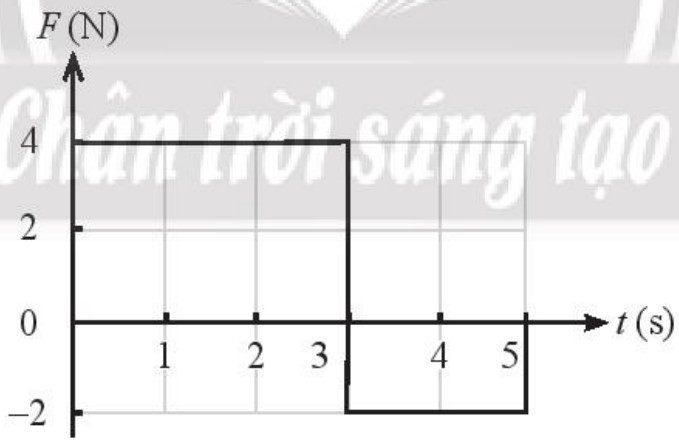
\includegraphics[scale=0.5]{../figs/VN10-2023-PH-TP029-P-1}
	\end{center}
	Xác định tốc độ của chất điểm tại các thời điểm:
	\begin{enumerate}[label=\alph*)]
		\item $t=\SI{3}{\second}$.
		\item $t=\SI{5}{\second}$.
	\end{enumerate}
	\loigiai{
	\begin{enumerate}[label=\alph*)]
		\item $\Delta p=F\cdot\Delta t\Rightarrow v_{t=\SI{3}{{\second}}}=\dfrac{F\cdot\Delta t}{m}=\SI{8}{\meter/\second}$.
		\item $\Delta p=F\cdot\Delta t\Rightarrow v_{t=\SI{5}{\second}}-v_{t=\SI{3}{\second}}=\dfrac{F\cdot\Delta t}{m}\Rightarrow v_{t=\SI{5}{\second}}=v_{t=\SI{3}{\second}}+\dfrac{F\cdot\Delta t}{m}\approx\SI{5.33}{\meter/\second}$.
	\end{enumerate}
	}
\end{ex}
\Closesolutionfile{ans}